\subsection{Autotuning and Caching\label{sec:autotuning}}

While the polyhedral core of TC is capable of optimizing and
generating code for any TC function, it is well known that the state
of the art linear optimization heuristics are not sufficient to
account for all performance anomalies and interactions with downstream
program transformations \cite{Zinenko2018Spatial,KongVocabulary}.
Different kernels need different, target-specific optimization trade-offs.
We thus complement our flow by an autotuner that varies the options of the
polyhedral JIT compiler marked as \emph{tunable} in the previous section.
These options can be stored and reused for similar
operations/kernels (similar shapes, target architecture) since autotuning may
require significantly more time than compilation.
% If polyhedral compilation becomes prohibitively expensive, it is possible to
% cache the produced CUDA or PTX code.

The tuning session is defined by a list of parameters to tune and
their admissible values, initial values, and the search strategy.  We
currently implement a genetic search strategy~\cite{Goldberg1989}.  It
runs for multiple steps, each one evaluating multiple candidate
values.  Each candidate is assigned a fitness value inversely
proportional to its runtime.  The pool is updated on each generation
by cross-breeding three candidates, chosen from the pool at random,
with fitter candidates having a higher chance of being chosen, such
that the each candidate's value is inherited from one of its parents.
A subsequent mutation phase can change the candidate's values at
random with some low probability. Much of the autotuning effort
resides in tile size selection, for which no linear objective
functions exist in polyhedral compilers. Genetic approaches have been
used successfully to explore such spaces, performing better than
random search due to the strong coupling of optimization
decisions---including tile sizes bound by the limits of the memory
hierarchy---\cite{Pou11,autotvm}.

Autotuning evaluates 100s to 1000s versions for each kernel.  We devise a
generic multi-threaded, multi-GPU autotuner.  It
maintains a queue of candidates to compile with the polyhedral flow, and a
queue of compiled kernels ready to be profiled on the GPU (see
\figref{comp_work_queue}).  Candidates or kernels are picked up by available
worker threads and compiled or profiled concurrently.  Profiling results are
accumulated in the tuning database and used for setting up successive search
steps.

\begin{figure}[h!tb]
  \centering
  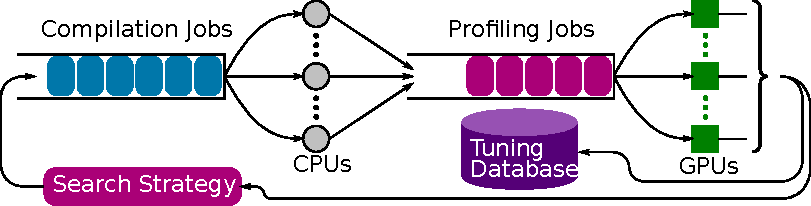
\includegraphics[width=.6\columnwidth]{extra/autotuner.pdf}
  \caption{Multithreaded autotuning pipeline for kernels}
  \label{fig:comp_work_queue}
\end{figure}

% Uncomment if have space
%
%The autotuner varies multiple options, among others it tunes:
%\begin{itemize}
%\item grid and block sizes, loop \emph{tiling} parameters (powers of 2 and
%integer ceil divisors of the problem size);
%\footnote{In our experience, for latency-bound kernels, it is often preferable
%to avoid launching an extra block for problem sizes close to a power of $2$
%(e.g., $130$) by using a slightly larger block size.}
%\item the bound on the number of iterations to \emph{unroll} (powers of 2 up to
%$256$);
%\item discrete choices on loop fusion, schedule shapes, promotion to shared
%memory and registers.
%\end{itemize}

Each generated version is ``warmed up'' by a few
executions before being profiled.  Without any performance guarantees,
autotuning needs to quickly prune poor candidates.  Because CUDA
kernels cannot be stopped once launched,
we rely on the following pruning heuristics to decrease the
autotuning time by an order of magnitude. (1) Parameter specialization
allows the exact number of active threads and blocks to be computed beforehand.
Kernels with fewer threads than some configurable threshold (e.g., $256$) are
not launched. (2) If during the first run, a kernel is more
than $100\times$ slower than the best version so far, or it is $5\times$ slower
after warmup, it is pruned immediately.

While autotuning time may become significant, compilation and
autotuning time is not a fundamental limit to TC's applicability.  In
training scenarios, a significant amount of time is spent on computing
the same kernel repeatedly over different data during the (stochastic)
gradient descent.  In inference scenarios, the network is optimized
ahead of time. As a result, although TC operates as a JIT compiler, it
only marginally hits the typical compilation/run-time trade-offs of
JIT compilers. Autotuning time may become an issue in specific
training scenarios where hyper-parameters would need to be frequently
updated, but in such a case one may leverage TC's intrinsic handling
of dynamic shapes and generate a single version of each operator or
fused operators to handle all hyper-parameter configurations.

%%Uncomment if have space
%In the future we plan to drive this pruning and, more generally, the search
%with a model but for the time being, we deem the user experience of our tuning
%flow satisfactory.
